\section{Det samlede system}\label{sec:samlet_system}
\textit{Dette afsnit omhandler test af det samlede system, hvis design og implementering består af indholdet fra de forrige blokke.}

Det samlede system består en række blokke, som tidligere er blevet designet, implementeret og testet for, hvorvidt disse blokke opfylder deres krav. Det fremgår af testene, at de separate blokke overholder de opstillede krav. Det samlede system sammensættes af hver enkelt blok og implementeres, som det fremgår af \figref{fig:design_blokdiagram} med undtagelse af pulsdetektering. 

\subsection{Test}
Testen udføres på baggrund af de opstillede krav og tilhørende afvigelser opstillet i \secref{krav_samlet_sys}. Kravene beskriver, at det samlede system skal:
\begin{itemize}
	\item Kunne detektere aktiviteterne gang, løb og cykling ved brug af et gyroskop og et accelerometer. Der accepteres ikke brug af andre sensorer.
	\item Automatisk kunne adskille gang, løb og cykling ved hjælp af algoritmer. Der accepteres en afvigelse på 10\% i forhold til fejlvurdering af aktivitet.
	\item Kunne detektere varighed fra systemets start. Der accepteres en afvigelse på 10\% i forhold til fejlvurdering af den samlede varighed.	
	\item Kunne detektere puls ved brug af pulssensor og tilhørende algoritme samt derefter kategorisere intensiteten af en given aktivitet. Der accepteres en afvigelse på 10\%.
	\item Videresende signaler til en ekstern enhed ved hjælp af BLE. Der accepteres ikke andre trådløse kommunikationsformer.
	\item Besidde batterilevetid for en hel dag svarende til 15 timer. Der accepteres ikke en batterilevetid på mindre end 15 timer.
	\item Repræsentere varigheden og pointfordelingen af en given aktivitet i GUI. Der accepteres ikke en anden form for visualisering.	
\end{itemize}
Kravet om registrering af puls vil ikke blive opfyldt, da pulssensoren ikke indgår i det samlede system, som beskrevet i \secref{sec_de_im_te_puls}. Det første krav om brug af accelerometer og gyroskop er opfyldt, da disse sensorer netop er valgt til formålet. Derudover er systemet designet til at sende via BLE, og en GUI bliver anvendt til visualisering. Derved overholdes disse krav ligeledes. \\
Formålet af testen af det samlede system er at undersøge, hvorledes de resterende krav overholdes. Det samlede systems funktionalitet testes ved først at opsætte softwaren på ICen og GAP peripheral ved brug af programmet PSoC. Derefter skal ICen sammensættes med GAP peripheral samt en spændingsforsyning til begge enheder og påføres en forsøgsperson. GAP central tilkobles en computer, hvorved denne MCU modtager resultater fra GAP peripheral. GAP peripheral kommunikerer trådløst via BLE med GAP central, hvorved data fra GAP central illustreres i GUI. Den perifere opsætning og montering fremgår af \figref{fig:samlede_system_opstilling}.
\begin{figure}[H]
	\centering
	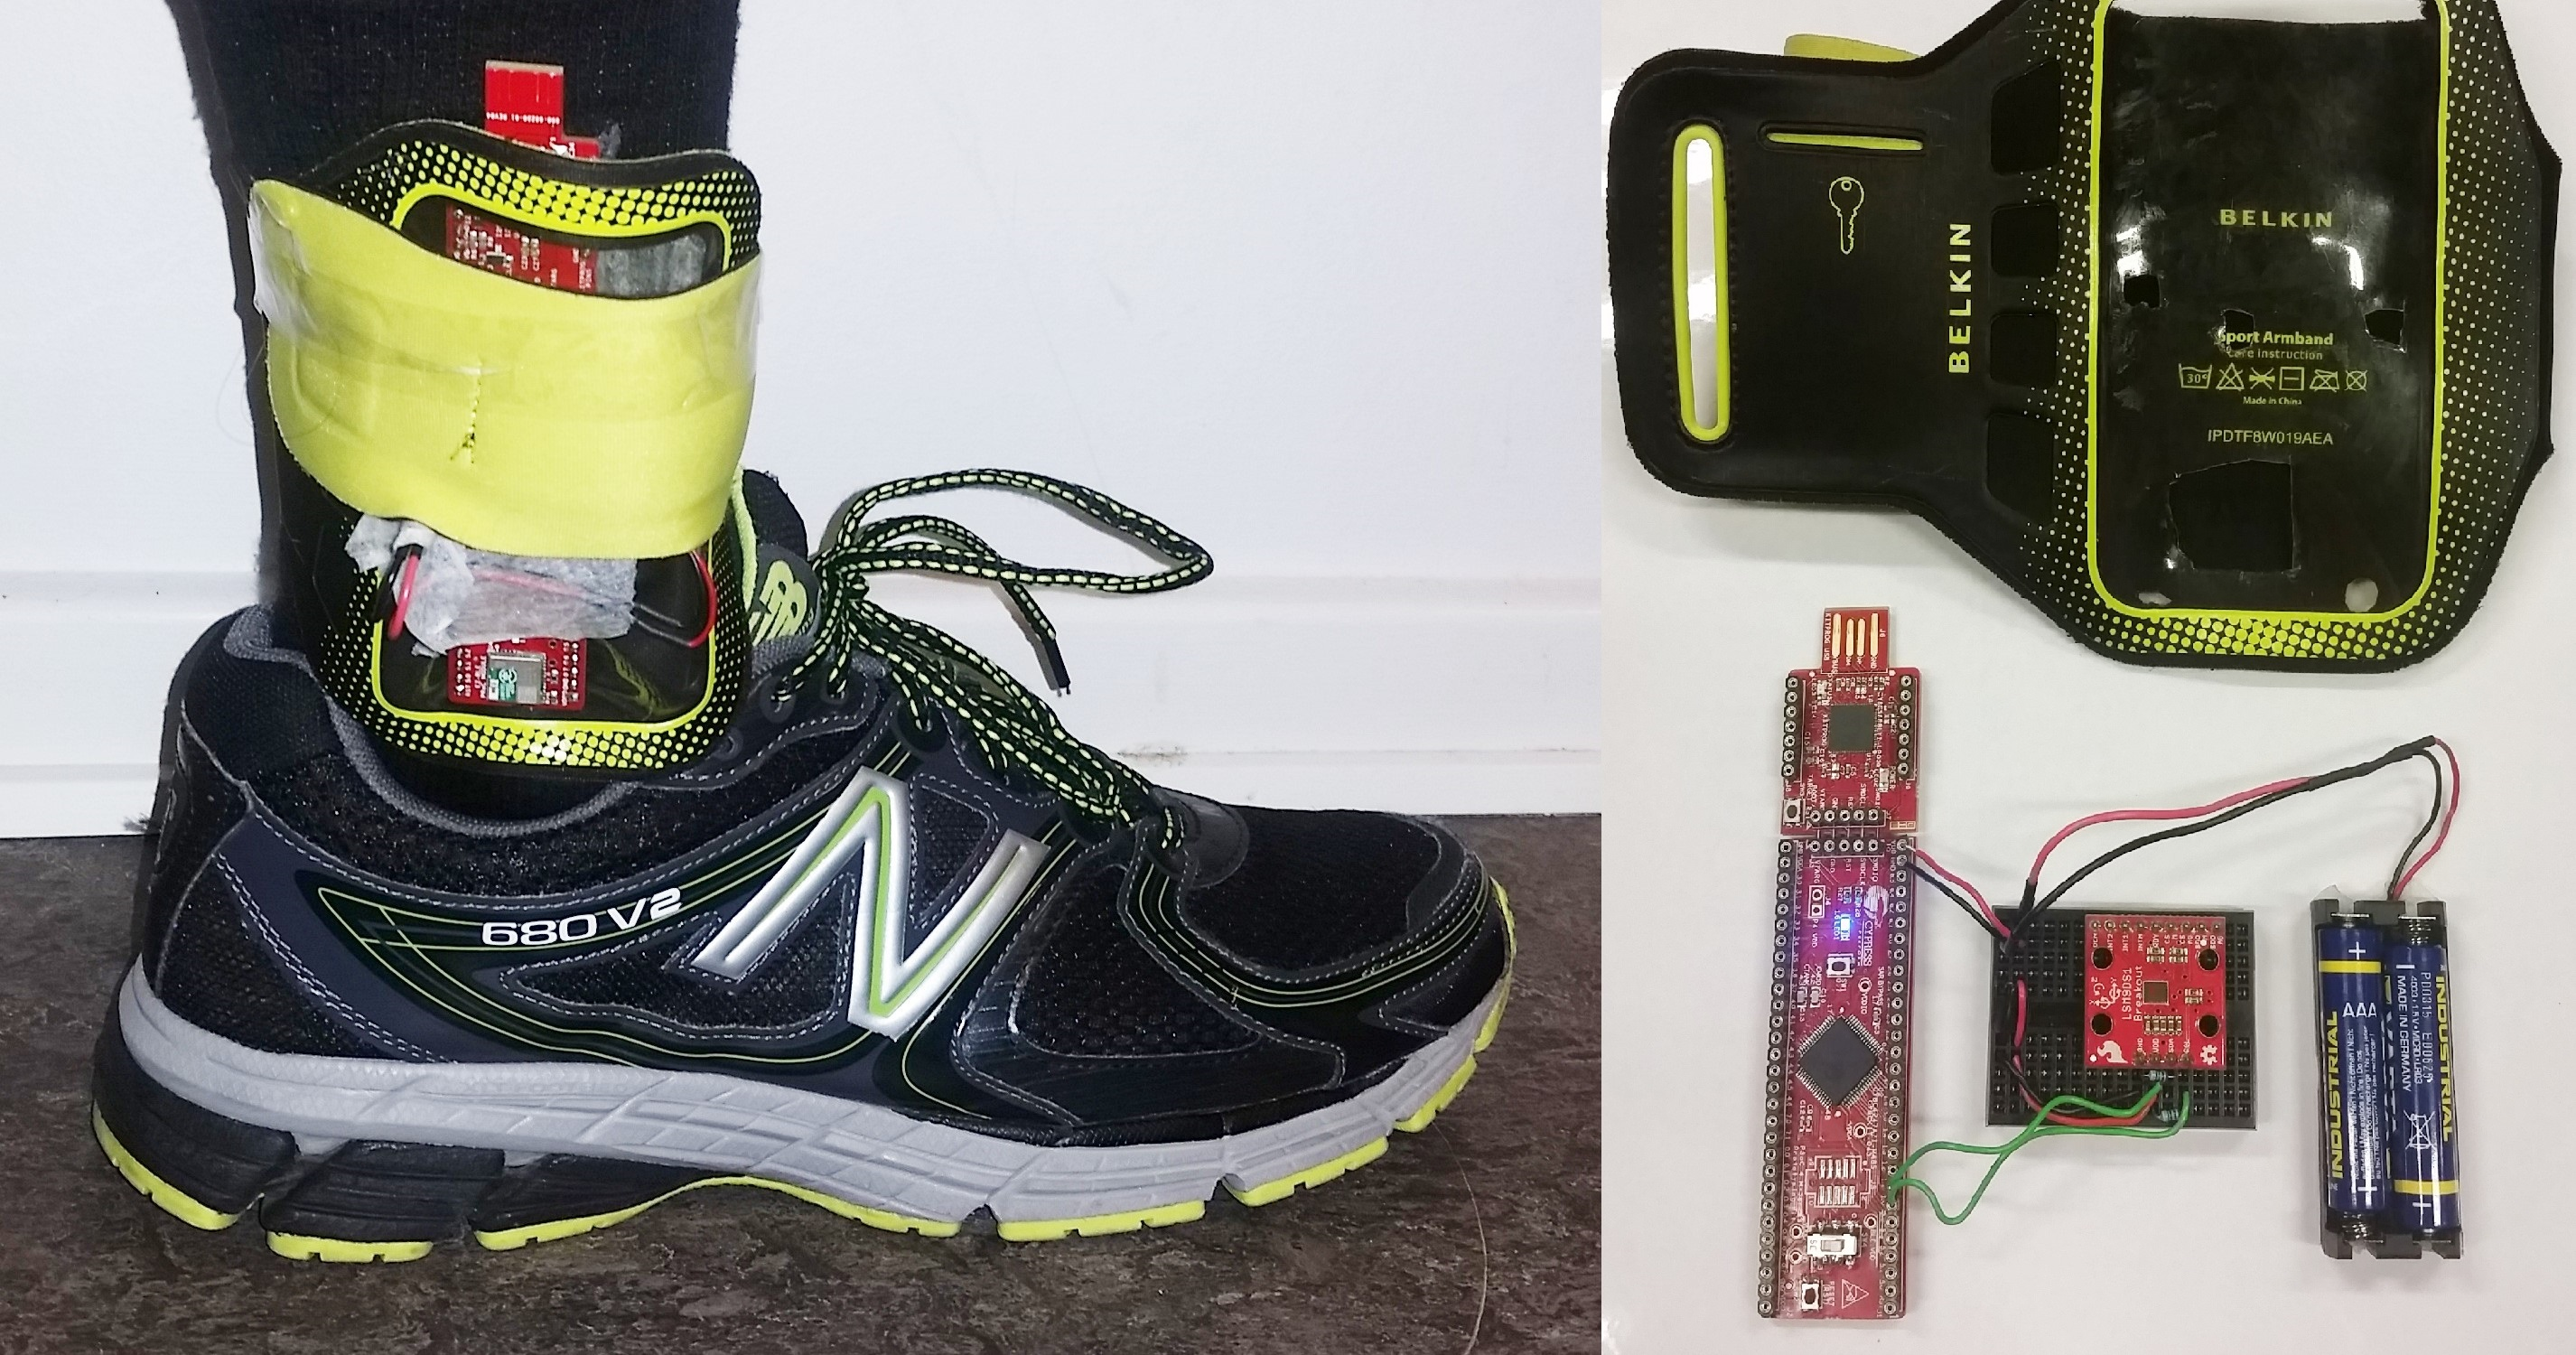
\includegraphics[scale=0.143]{figures/cDesign/samlet_system_paafod4.jpg}
	\caption{På figuren ses henholdsvis opsætningen af den perifere del af det endelige system på en forsøgsperson samt det samlede system taget ud af holderen. Der ses, at EZ\_BLE modulet er frit tilgængeligt i bunden til venstre i selve opsætningen.}
	\label{fig:samlede_system_opstilling}
\end{figure}\vspace{-.25cm}
Ved test af det samlede system skal en forsøgsperson udføre tre aktiviteter: gang med 4,8 km/t, løb med 11,3 km/t og cykling med 20,9 km/t. Hver aktivitet skal udføres i 60 sekunder, og dataopsamlingen skal påbegyndes, når forsøgspersonen vurderer at have en homogen cyklus. Forinden tages en 60 sekunders måling, hvor forsøgspersonen står stille på løbebåndet. Fremgangsmåden for første test af systemet med gang ses herunder: 
\begin{itemize}
\item GAP peripheral med IC og en spændingsforsyning placeres proximalt for den laterale malleolus, som ses på \figref{fig:samlede_system_opstilling}.
\item GAP central kobles til en computer.
\item Forsøgspersonen skal opnå en homogen cyklus på løbebåndet, som indstilles til 4,8 km/t. 
\item Et stopur startes samtidig med GUI.
\item Efter 60 sekunder på stopuret stoppes målingen.
\end{itemize}
Dette forsøg udføres for gang og løb, hvorefter testen vedrørende cykling udføres. Fremgangsmåden er tilsvarende for cykling, hvoraf denne aktivitet udføres på en motionscykel. Resultatet fra denne test forekommer som en fordeling af aktiviteter i GUIen, som ikke bør opfange andre aktiviteter end den udførte aktivitet. GUI bør ligeledes registrere 60 sekunder af hver aktivitet, hvis algoritmen fungerer efter hensigten. \\
Resultatet fra de forskellige tests ses i \tabref{tab:samlet_sys_test1}
\begin{table}[H]
	\centering
	\resizebox{\textwidth}{!}{%
	\begin{tabular}{ccccccc}
			\cellcolor[HTML]{C0C0C0}Aktivitet & 	\cellcolor[HTML]{C0C0C0} Forsøgsperson & 	\cellcolor[HTML]{C0C0C0}\begin{tabular}[c]{@{}c@{}} Detektion af \\ gang {[}s{]} \end{tabular} & 	\cellcolor[HTML]{C0C0C0}\begin{tabular}[c]{@{}c@{}} Detektion af \\ løb {[}s{]} \end{tabular} & \cellcolor[HTML]{C0C0C0}\begin{tabular}[c]{@{}c@{}} Detektion af \\ cykling {[}s{]} \end{tabular} & \cellcolor[HTML]{C0C0C0}\begin{tabular}[c]{@{}c@{}} Afvigelse i detektering\\ af aktivitet {[}\%{]} \end{tabular} & \cellcolor[HTML]{C0C0C0}\begin{tabular}[c]{@{}c@{}} Afvigelse af varighed \\ på 60 sekunder {[}\%{]} \end{tabular} \\ \hline
        \multirow{5}{*}{Gang}                                                     & F1             & 39,9                                                                                                & 1,1                                                                                              & 0  & 2,8   & -31,7                                                                                                \\
		& F2             & 40,6                                                                                                & 0                                                                                                & 0   & 0      & -32,3                                                                                            \\
		& F3             & 39                                                                                                  & 2                                                                                                & 0       & 5,1    & -31,7                                                                                          \\
		& F4             & 39,7                                                                                                & 1,6                                                                                              & 0      & 4   & -31,2                                                                                           \\
		& F5             & 40,8                                                                                                & 0                                                                                                & 0      & 0    & -32                                                                                          \\ \hline
		\multirow{5}{*}{Løb}                                                      & F1                                                                                                          & 1,2 & 39,9                                                                                             & 0     & 3 & -31,5                                                                                               \\
		& F2                                                                                           & 1,8  & 39                                                                                            & 0         & 4,6     & -32                                                                                       \\
		& F3                                                                                              & 0    & 40,8                                                                                            & 0      & 0         & -32                                                                                      \\
		& F4                                                                                                      & 0,4  & 40,4                                                                                            & 0     & 1    & -32                                                                                           \\
		& F5                                                                                                    & 0     & 40,6                                                                                           & 0         & 0 & -32,3  \\ \hline
		\multirow{5}{*}{Cykling}     & F1     & 0        & 0     & 40    & 0    & -33,3  \\ 
		& F2             & 0                                                                                                & 0                                                                                                & 40       & 0 & -33,3                                                                                             \\
		& F3             & 0                                                                                                  & 0                                                                                                & 40      & 0   & -33,3                                                                                           \\
		& F4             & 0                                                                                                  & 0                                                                                                & 40    & 0   & -33,3                                                                                              \\
		& F5             & 0                                                                                                  & 0                                                                                                & 36 & 0 & -40  \\ \hline                                                                                                
		\end{tabular}
	}
		\caption{I tabellen ses resultaterne fra de tre tests af det samlede system. Derudover er afvigelsen for hver detektion af fysisk aktivitet samt samlet varighed udregnet.}
		\label{tab:samlet_sys_test1}
\end{table}\vspace{-.25cm}
Der ses i \tabref{tab:samlet_sys_test1}, at GUIen hovedsageligt optager den pågældende aktivitet. Ved målingen, hvor der ikke blev udført en aktivitet, bliver der ikke detekteret nogen aktivitet i GUIen. Dette fremgår imidlertid ikke i \tabref{tab:samlet_sys_test1}. \\
Overordnet for detekteringen af aktiviteterne er den største afvigelse på 5,13\%. Dermed overholder systemet kravet om, at der må være en maksimal afvigelse på 10\% i forhold til detektion af aktivitet. Der ses dog også i \tabref{tab:samlet_sys_test1}, at GUIen detekterer cirka 40 sekunders data $\pm$1 sekund, selvom dataopsamlingen varer i 60 sekunder. Dette giver en maksimal afvigelse på -40\% af den totale detekterede varighed i forhold til varigheden fra systemets start. Systemet overholder dermed ikke kravet om, at der må være en maksimal afvigelse på 10\% i forhold til detektering af varighed.

Der foretages yderligere en test af systemet, hvor forsøgspersonerne først skal forsøge at gå ved en bestemt hastighed og derefter løbe ved samme hastighed. Derved testes systemet ved en hastighed, som både kan være gang og løb, for at undersøge systemets reaktion herfra. Fremgangsmåden for testen er tilsvarende forrige test, hvor hastigheden til denne test er 8 km/t. Hastigheden vælges på baggrund af pilotforsøget samt studier. I pilotforsøget skiftede hver forsøgsperson fra gang til løb under hastighedsstigningen mellem 8 og 10 km/t. Derudover hævder studier, at 6,4~km/t svarer til rask gang mens 9,7~km/t er langsomt løb. 8 km/t vælges derfor, da denne hastighed ligger mellem gang og løb. \citep{Miles2007} Resultatet fra denne test ses i \tabref{tab:samletsys_8kmt}
\begin{table}[H]
	\centering
		\resizebox{\textwidth}{!}{%
	\begin{tabular}{ccccccc}
		\cellcolor[HTML]{C0C0C0}\begin{tabular}[c]{@{}c@{}} Aktivitet \\ ved 8 km/t\end{tabular} & 	\cellcolor[HTML]{C0C0C0} Forsøgsperson & 	\cellcolor[HTML]{C0C0C0}\begin{tabular}[c]{@{}c@{}} Detektion af \\ gang {[}s{]} \end{tabular} & 	\cellcolor[HTML]{C0C0C0}\begin{tabular}[c]{@{}c@{}} Detektion af \\ løb {[}s{]} \end{tabular} & \cellcolor[HTML]{C0C0C0}\begin{tabular}[c]{@{}c@{}} Detektion af \\ cykling {[}s{]} \end{tabular} & \cellcolor[HTML]{C0C0C0}\begin{tabular}[c]{@{}c@{}} Afvigelse i detektering\\ af aktivitet {[}\%{]} \end{tabular}  & \cellcolor[HTML]{C0C0C0}\begin{tabular}[c]{@{}c@{}} Afvigelse af varighed \\ på 60 sekunder {[}\%{]} \end{tabular}\\ \hline 
		\multirow{5}{*}{Gang}                                                     & 1             & 36,3                                                                                                & 4,3                                                                                              & 0  & 11,9   & -32,3                                                                                                \\
		& 2             & 31,1                                                                                                & 9,9                                                                                                & 0   & 31,8  & -31,7                                                                                                \\
		& 3             & 2,3                                                                                                  & 38,3                                                                                                & 0       & 94,3 & -32,3                                                                                            \\
		& 4             & 4                                                                                                & 36,7                                                                                              & 0      & 90,2& -32,2                                                                                               \\
		& 5             & 0,4                                                                                                & 40,4                                                                                                & 0      & 99 & -32                                                                                              \\ \hline
		\multirow{5}{*}{Løb}                                                      & 1                                                                                                          & 0,8 & 40                                                                                             & 0     & 2   & -32                                                                                             \\
		& 2                                                                                           & 0,9  & 40                                                                                            & 0         & 2,3 & -31,8                                                                                           \\
		& 3                                                                                              & 2,3    & 38,6                                                                                            & 0      & 6 & -31,8                                                                                              \\
		& 4                                                                                                      & 0,2  & 40,7                                                                                            & 0     & 0,5   & -31,8                                                                                             \\
		& 5                                                                                                    & 0,9     & 40,2                                                                                           & 0         & 2,2 & -31,5  \\ \hline 
		\end{tabular}
	}
	\caption{I tabellen ses resultaterne fra en test, hvor forsøgspersonerne skulle henholdsvis gå eller løbe ved samme hastighed. Der ses yderligere, at afvigelserne ved en mellemting mellem gang og løb er betydeligt mere signifikante, end ved klar gang eller løb. Dette går især ud over detektering af aktiviteten gang.}
	\label{tab:samletsys_8kmt}
\end{table}\vspace{-.25cm}
Der ses i \tabref{tab:samletsys_8kmt}, at når hastigheden for aktiviteten ikke er klar gang eller løb for forsøgspersonen, så vil den procentvise afvigelse stige markant vedrørende resultatet for gang. Dette grunder i, at 8 km/t vurderes som værende meget rask gang fra hver forsøgsperson. Derfor vil g-påvirkningen af accelerometerets y-akse også blive påvirket med mere kraft end ved normal gang. Der ses, at forsøgsperson 1 og 2 har lavere afvigelse for gangsignalet end forsøgsperson 3 til 5.

Afslutningsvis testes spændingsforbruget af den eksterne spændingsforsyning, som beskrevet i \secref{spaendingsforsyning}. Testen foregår således, at den eksterne spændingsforsyning indeholder nyudskiftede batterier og herefter måles outputspændingsniveauet. Efterfølgende bliver spændingsforbruget målt hver halve time under den samlede systemtest. Der antages, at spændingsforbruget er lineært faldende, hvorfor en gennemsnitsværdi for spændingsforbruget per time udregnes. \\
Spændingsforsyningen leverede 3,19 V fra starten af testen. Resultatet af de efterfølgende fem målinger ses i \tabref{tab:samlet_sys_batteri}
\begin{table}[H]
	\centering
	\begin{tabular}{ccc}
		\hline
		\cellcolor[HTML]{C0C0C0}Tid {[}t{]} & \cellcolor[HTML]{C0C0C0} Spændingsniveau {[}V{]} & \cellcolor[HTML]{C0C0C0}Spændingsforbrug {[}V{]} \\ \hline
		0 & 3,19 & 0 \\ \hline	
		0,5 & 3,104 & 0,086 \\ \hline	
		1 & 3,052 & 0,052 \\ \hline
		1,5 & 3,016 & 0,036 \\ \hline
		2 & 2,969 & 0,047 \\ \hline
		2,5 & 2,951 & 0,018 \\ \hline
	\end{tabular}
	\caption{I tabellen ses resultatet fra målingerne af spændingsforbruget for den eksterne spændingsforsyning. Der ses yderligere det beregnede spændingsforbrug for hver måling.}
	\label{tab:samlet_sys_batteri}
\end{table}\vspace{-.25cm}
I \tabref{tab:samlet_sys_batteri} ses spændingsforbruget over fem målinger med en halv times interval. Det antages, at spændingsforbruget har et lineært forhold, bliver en gennemsnit beregnet i \eqref{eq:samlet_sys1}.
\begin{equation}
\frac{(0,086 + 0,052 + 0,036 + 0,047 + 0,018)~V}{5 \text{målinger}} \cdot 2 = \text{0,0956~V/t}
\label{eq:samlet_sys1}
\end{equation}
Med antagelse af lineært forhold vil spændingsforsyningen falde med 0,0956 V per time. Spændingen ved start er 3,19 V og den endelige spænding, hvormed MCUen ikke længere er funktionel, er 1,71 V. Det maksimale spændingsinterval er derfor $3,19~V - 2,40~V = 0,79~V$. Derfor er levetiden for den eksterne spændingsforsyning udregnet til:
\begin{equation}
\frac{0,79~V}{0,0956~V/t} = \text{8,3~t}
\label{eq:samlet_sys2}
\end{equation}
I \eqref{eq:samlet_sys2} ses det, at den eksterne spændingsforsyning teoretisk kan få det samlede sytem til at være funktionel i 8,3 timer. Derfor overholder det samlede system ikke kravet om, at det skal besidde batterilevetid i op til 15 timer. 